\documentclass[12pt,a4paper]{article}

\usepackage{amsmath, amssymb, tikz, geometry, tabularx, array}
\geometry{margin=1in}
\setlength{\parskip}{6pt}

\title{Vector Worksheet --- Worked Solutions}
\author{}
\date{}

\begin{document}
\maketitle
\thispagestyle{empty}

\section*{Vector Representations}

For a vector from \(P\) to \(Q\),
\[
\overrightarrow{PQ}
=
\begin{pmatrix}
x_Q-x_P\\
y_Q-y_P
\end{pmatrix}.
\]

For \(\mathbf{v}\), the column vector is already given as
\(\begin{pmatrix}5\\3\end{pmatrix}\), so
\[
Q=P+\begin{pmatrix}5\\3\end{pmatrix}
=(2,3)+(5,3)=(7,6).
\]

For \(\mathbf{w}\),
\[
\overrightarrow{CD}
=
D-C
=
\begin{pmatrix}1-(-3)\\5-2\end{pmatrix}
=
\begin{pmatrix}4\\3\end{pmatrix}.
\]

For the own example \(\mathbf{t}\), choose
\[
Y=(8,3).
\]
Then
\[
\overrightarrow{XY}
=
\begin{pmatrix}8-5\\3-0\end{pmatrix}
=
\begin{pmatrix}3\\3\end{pmatrix}.
\]

\begin{center}
\small
\begin{tabularx}{\textwidth}{|>{\raggedright\arraybackslash}p{2.4cm}|>{\centering\arraybackslash}p{2.4cm}|>{\centering\arraybackslash}p{2.4cm}|>{\centering\arraybackslash}p{2.4cm}|>{\centering\arraybackslash}p{2.4cm}|}
\hline
& \(\mathbf{u}\) & \(\mathbf{v}\) & \(\mathbf{w}\) & \(\mathbf{t}\) (own) \\
\hline
Points
&
\(A=(0,0)\), \(B=(3,-1)\)
&
\(P=(2,3)\), \(Q=(7,6)\)
&
\(C=(-3,2)\), \(D=(1,5)\)
&
\(X=(5,0)\), \(Y=(8,3)\)
\\
\hline
Directed path
&
\(\overrightarrow{AB}\)
&
\(\overrightarrow{PQ}\)
&
\(\overrightarrow{CD}\)
&
\(\overrightarrow{XY}\)
\\
\hline
Column vector
&
\(\begin{pmatrix}3\\-1\end{pmatrix}\)
&
\(\begin{pmatrix}5\\3\end{pmatrix}\)
&
\(\begin{pmatrix}4\\3\end{pmatrix}\)
&
\(\begin{pmatrix}3\\3\end{pmatrix}\)
\\
\hline
\end{tabularx}
\end{center}

\section*{Adding Vectors}

Many routes are possible. One valid route through the grey track is shown below.

Start at
\[
R=(-9,-3).
\]
Apply the vector
\[
\mathbf{g}=\begin{pmatrix}1\\3\end{pmatrix}.
\]
Then the endpoint is
\[
S=R+\mathbf{g}=(-9,-3)+(1,3)=(-8,0).
\]

The route crosses the Start/Finish line when \(y=-1\). Since
\[
R+t\mathbf{g}=(-9,-3)+t(1,3),
\]
we solve
\[
-3+3t=-1 \implies t=\frac23.
\]
At that point,
\[
x=-9+\frac23=-\frac{25}{3}\approx -8.33,
\]
which lies on the Start/Finish line segment between \((-10,-1)\) and \((-8,-1)\). The whole segment stays inside the grey track; the endpoint \((-8,0)\) touches the inner edge, which is allowed.

\begin{center}
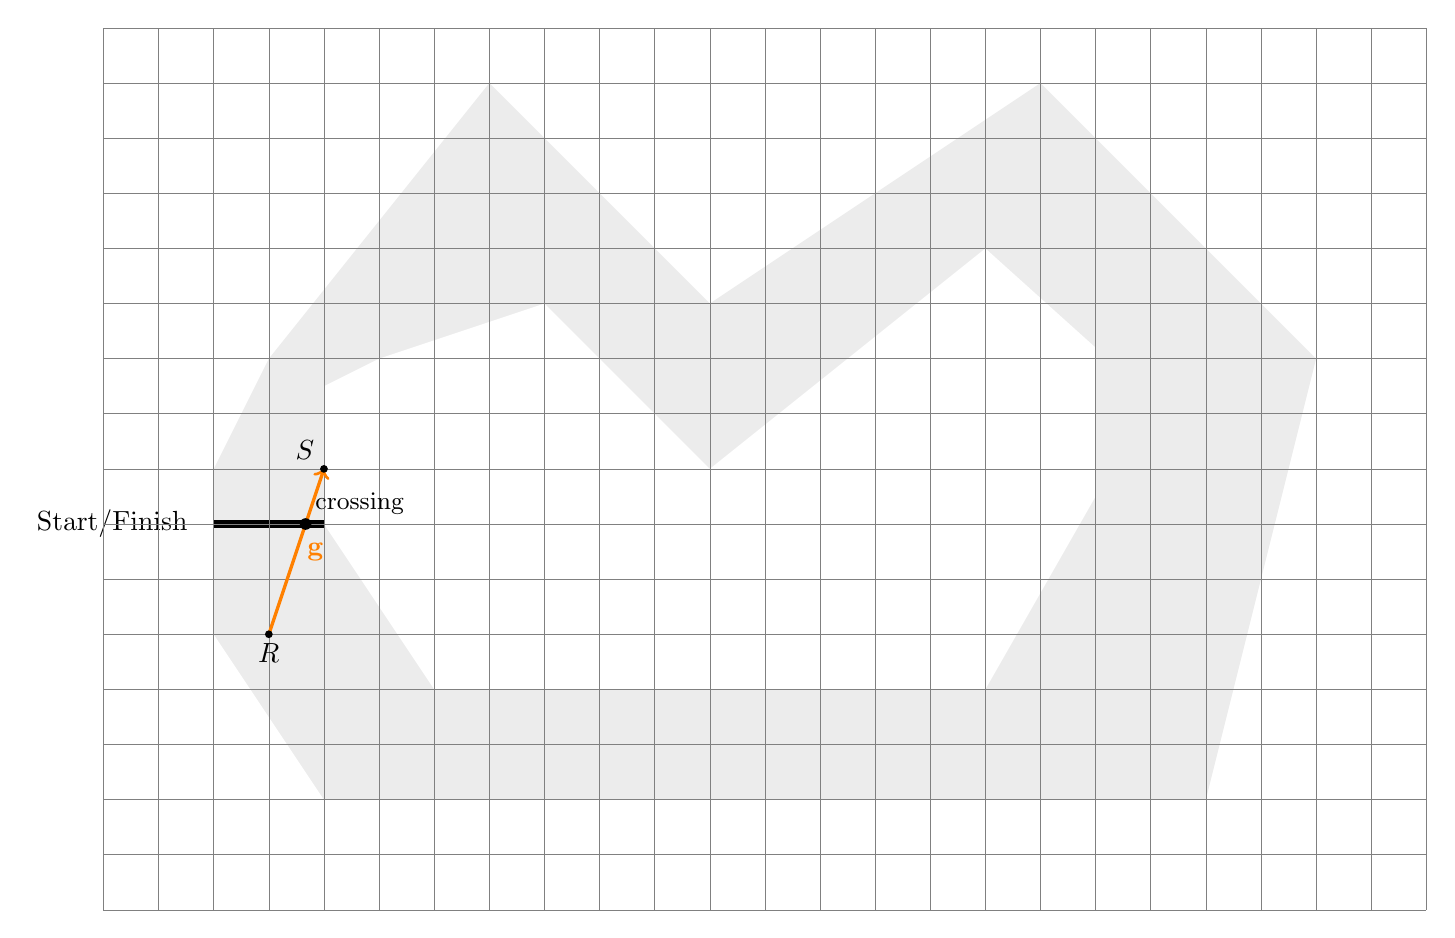
\begin{tikzpicture}[scale=0.7]
    % Inner boundary
    \draw[line width=3pt, rounded corners=26pt]
        (-8,-1)
        -- (-6,-4)
        -- (3,-4)
        -- (3,-2.5)
        -- (6,2.2)
        -- (3.2,4)
        -- (-1,2)
        -- (-4,4)
        -- (-7,2)
        -- (-8,1.5)
        -- cycle;

    % Track fill
    \begin{scope}
        \clip (-10,-3)
            -- (-8,-6)
            -- (8,-6)
            -- (9,-2)
            -- (10,2)
            -- (5,7)
            -- (-1,3)
            -- (-5,7)
            -- (-9,2)
            -- (-10,0)
            -- cycle;

        \fill[gray!15] (-12,-8) rectangle (12,8);

        \fill[white]
            (-8,-1)
            -- (-6,-4)
            -- (4,-4)
            -- (6,-0.5)
            -- (6,2.2)
            -- (4,4)
            -- (-1,0)
            -- (-4,3)
            -- (-7,2)
            -- (-8,1.5)
            -- cycle;
    \end{scope}

    % Start/Finish line
    \draw[line width=3pt] (-10,-1) -- (-8,-1);
    \node[anchor=east] at (-10.3,-1) {Start/Finish};

    % Grid
    \draw[help lines, step=1] (-12,-8) grid (12,8);

    % Worked route
    \draw[->, very thick, orange] (-9,-3) -- (-8,0)
        node[midway, right] {\(\mathbf{g}\)};

    \fill (-9,-3) circle (2pt) node[below] {\(R\)};
    \fill (-8,0) circle (2pt) node[above left] {\(S\)};
    \fill (-8.333,-1) circle (3pt) node[above right] {\small crossing};
\end{tikzpicture}
\end{center}

\begin{enumerate}
    \item Write your path in the form \(g + a + \cdots\)
    \[
    \boxed{\mathbf{g}}
    \]

    \item Collect the like terms in your expression.

    Since only \(\mathbf{g}\) is used, there are no like terms to collect. The expression is already simplified:
    \[
    \mathbf{g}.
    \]

    \item Thus evaluate the expression from 1. as a column vector. What do you notice?

    \[
    \mathbf{g}=\begin{pmatrix}1\\3\end{pmatrix}.
    \]

    The resultant column vector is the total displacement from \(R\) to \(S\). It is exactly the column vector for \(\mathbf{g}\), because the route consists of a single application of \(\mathbf{g}\).
\end{enumerate}

\end{document}